\subsection{Evaluation}
\label{Evaluation}

In the following, I will evaluate the outcome of my optimizational work. Using experimental benchmark data, I will discuss the impact of the optimizations on the three algorithms and reason about the influence of anchor positions on each algorithm's performance. I will also debate the statistical significance of these benchmarks.

\subsubsection{Approach}
As mentioned in Section~\ref{benchmarking}, the following data has been collected using my custom-made \emph{benchlat} utility. For this final benchmark, the algorithms were executed 500 times each, using 3, 4, and 5 anchors for AML and VBLE-OPT, and only 3 anchors for Geo3, which simply discards additional anchors. Regarding the selection of anchor positions, I decided to mainly choose points close to distinct borders of the playing field, aiming at a near uniform distribution of the area of the shapes formed by the anchors, and at avoiding having a bias towards small, centered shapes that would arise from a uniform distribution of points. This can in general be considered more realistic for localization scenarios. Though, since the input parameters are discretized to integer simulation units by the engine, this constraint also resulted in a lower bound on the area of the anchor shape. For example, one minimal triangle would be formed by three points lying as close as possible to one border of the playing area without being colinear, for example, the points (1|0), (0|500), and (1|1000). This triangle still has an area of 500 square simulation units. However, I do not consider these (unlikely) minimum area shapes to be of major relevance for the speed-ups resulting from the optimization.

For each set of anchors, the original implementation of each algorithm was executed as well, in order to obtain a reference runtime. Both the reference and the optimized runtimes were reduced by the constant overhead imposed by the engine itself, which is mainly composed by the time it takes the engine to calculate the real distances and to generate the random measuring errors. In order to estimate this overhead, I executed the \emph{const} algorithm shipped with LS$^{2}$, which does nothing but return the input parameters, a thousand times and calculated the average of the runtimes. The resulting average overhead is 0.06603 seconds. 

The achieved speed-up of each anchor and algorithm combination was calculated using Formula 1 shown below, where $t_{o,i}$ denotes the optimized runtime and $t_{r,i}$ is the reference runtime. The average speed-up was derived using the usual formula for the arithmetic mean that is displayed in Formula 2.

\begin{align}
s_{i}& = \frac{t_{r,i}}{t_{o,i}} \\
\texttt{average}& = \frac{1}{n} \cdot \sum_{i = 1}^n s_{i}
\end{align}

The benchmarks were run on a quad-core Intel Xeon E31245 CPU with a clock frequency of 3.30~GHz, which had access to a total of 8~GB main memory. Because availability of this system was temporally limited, the number of algorithm iterations for each position needed to be reduced to 40, though, as execution runtimes are linearly dependent on the number of iterations (refer to Section~\ref{ls2}, this does not compromise the significance of the benchmark results. The framework was configured to always use uniformly distributed errors. This, by contrast, limits the universality of the benchmark results to some degree. However, at the time of my coding it was the only error model implemented in LS$^{2}$. The application was compiled using the GNU compiler collection, version 4.6.3, with compiler optimization set to \texttt{-O3}.

\subsubsection{Discussion}
To begin with, all benchmark runs have delivered a positive result, i.e., the performance of each algorithm has been improved no matter where the anchors were placed. Table~\ref{average_table} shows the average speed-up calculated over all benchmark runs for each algorithm for 3, 4, and 5 anchors, providing a convenient overview of how much the algorithms benefitted from the optimization. AML boasts the best results with an average speed-up of 2.7 to 3.0, followed by Geolateration and VBLE-OPT.

\begin{table}[ht]
\begin{center}
\caption{Average speed-ups}
\begin{tabular}{lccc} 
\toprule
& \multicolumn{3}{c}{Average speed-up} \\ 
\cmidrule(r){2-4}
Algorithm & 3 anchors & 4 anchors & 5 anchors \\
\midrule
AML & 3.30 & 3.34 & 3.36 \\
GEO3 & 2.20 & N/A & N/A \\ 
VBLE-OPT & 1.68 & 1.77& 1.75 \\
\bottomrule
\end{tabular}
\label{average_table}
\end{center}
\end{table}

Most prominently, the AML speed-ups seem to increase linearly, which was affirmed by (less numerous) experiments I conducted with 6 to 8 anchors. This is likely caused by the growing influence of the \emph{refinement} step, that could be perfectly vectorized due to the absence of conditional statements and thus has a considerable advantage over the scalar implementation. Using fewer anchors, the \emph{first intersection} step becomes the prevalent factor limiting the overall performance. However, as mentioned in the introduction, the theoretical speed-up of a SSE-based optimization is the number of vector elements, which is 4. I therefore suspect this increase to slowly decline with additional anchors until the speed-up factor has reached its peak, where it will probably stagnate or maybe start to decline due to other effects such as memory bandwidth limits.

\begin{figure}
\begin{center}
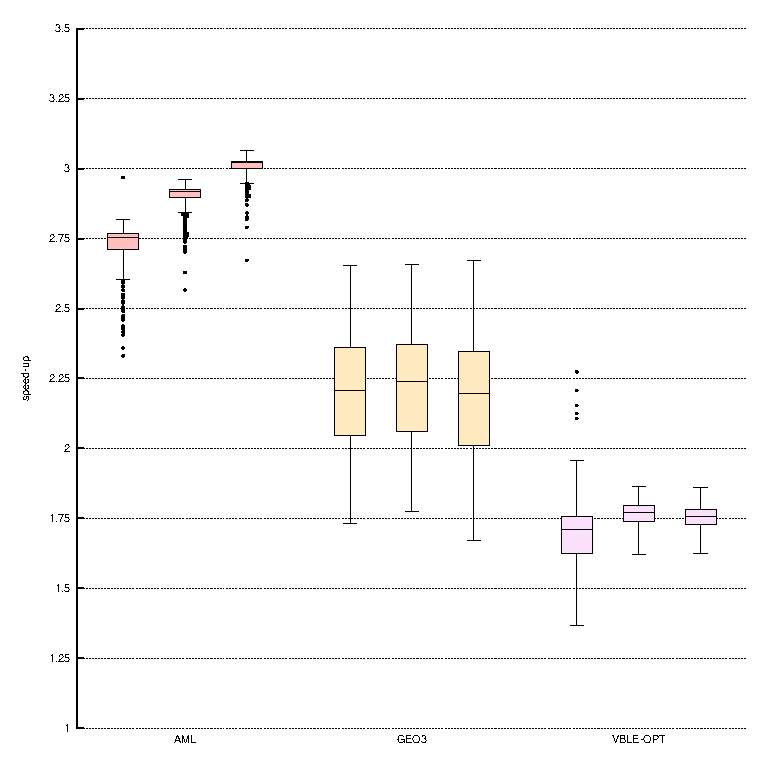
\includegraphics{img/boxplot}
\end{center}
\caption{Distribution of speed-ups}
\label{fig:boxplot}
\end{figure}

In general, it is arguable whether these average speed-ups can be used to evaluate the success of my optimizational work. The algorithms showed remarkable differences in the distribution of the test data, which can be seen in the box-and-whisker diagram in Figure~\ref{fig:boxplot}. Whereas speed-ups of AML and VBLE-OPT have a small variance, Geolateration has a considerably larger dispersion with its interquartile range spreading from around 2.05 to 2.35. I expect this to a be consequence of the many early-out conditionals contained in Geo3, which in general lead to large variances in the algorithm runtimes. Some manual investigation into the anchor placements for speed-ups both from the lower and from the upper range of results suggested that input anchors forming a large triangle (e.g., anchors lying close to distinct corners of the playing area) led to higher speed-ups, whereas small, acute-angled triangles resulted in lower speed-ups. In the latter case, the optimizational step 4, which tests whether the minimum perimeter triangle is contained in the triangle formed by the anchors, is more likely to fail and therefore the remaining parts are executed more often. This also shows that the overall speed-up of Geo3 is not cumulative over the performance improvements of the various sections: Whereas the optimization of step 5, which calculates the geometric median of the final triangle, proved highly beneficial in my experiments, the overall speed-up of the optimization is higher in cases where it is executed less frequently.

To put some visual emphasis on the distribution of the speed-ups with respect to the spread of the runtimes, Figures~\ref{fig:scatterplots}~and~\ref{fig:vblescatterplots} display scatterplots that relate the reference runtimes to the corresponding optimized runtimes, where each point represents a single pair of runtimes. The position of points relative to the x-axis shows the general variance of reference runtimes for the given 500 random benchmark runs. Additionally, the scattering of points around the green line, which interpolates the expected optimized runtimes using the calculated average speed-up (i.e., it is a plot of the formula $y = \frac{x}{\texttt{average speed-up}}$), illustrates the variance of the speed-ups. For example, to verify what has been said above, the upper right region of Figure~\ref{fig:scattergeo} shows that higher runtimes of Geo3 had an lower-than-average speed-up.

\begin{figure}
\begin{center}
\subfigure[Geo3]{
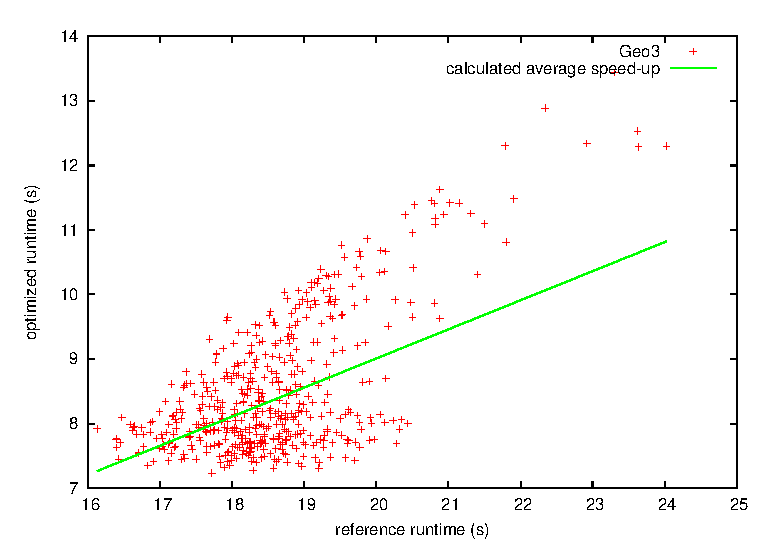
\includegraphics[width=0.75\linewidth]{img/scatter_geolat3.eps}
\label{fig:scattergeo}
}
\subfigure[AML (4 anchors)]{
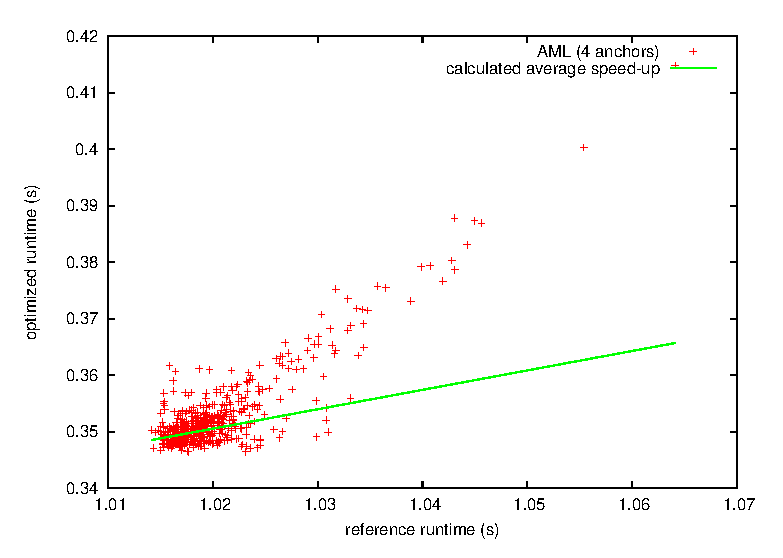
\includegraphics[width=0.75\linewidth]{img/scatter_aml4.eps}
\label{fig:scatteraml}
}
\end{center}
\caption*{\small{These scatterplots show the reference runtimes in relation to the corresponding optimized runtimes, so each point actually marks two measured values. The green line is an interpolation of the \emph{calculated average speed-up}, i.e. it can be read as, ``Based on the average speed-up, one can expect a run of the algorithm that took $x$ seconds in the original implementation to take $y$ seconds in the optimized version''.}}
\caption{Scatterplots of benchmark results}
\label{fig:scatterplots}
\end{figure}

\begin{figure}
\begin{center}
\subfigure[3 anchors]{
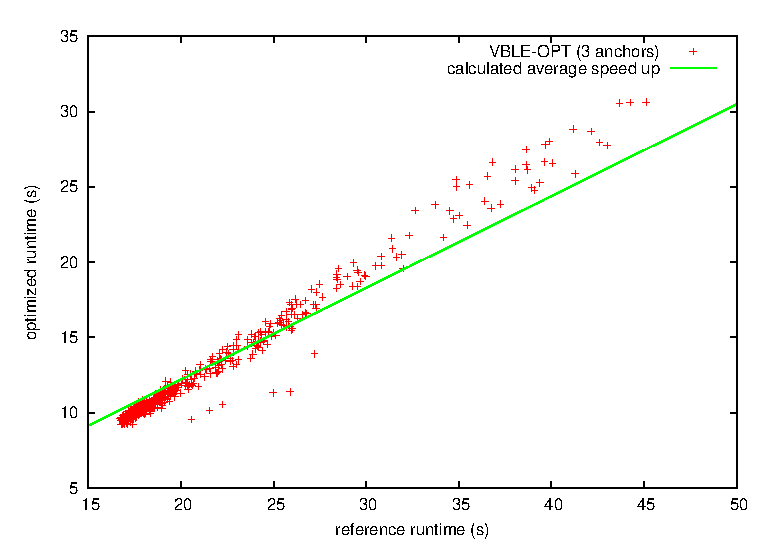
\includegraphics[width=0.75\linewidth]{img/scatter_vble3.eps}
\label{fig:scattervble3}
}
\subfigure[4 anchors]{
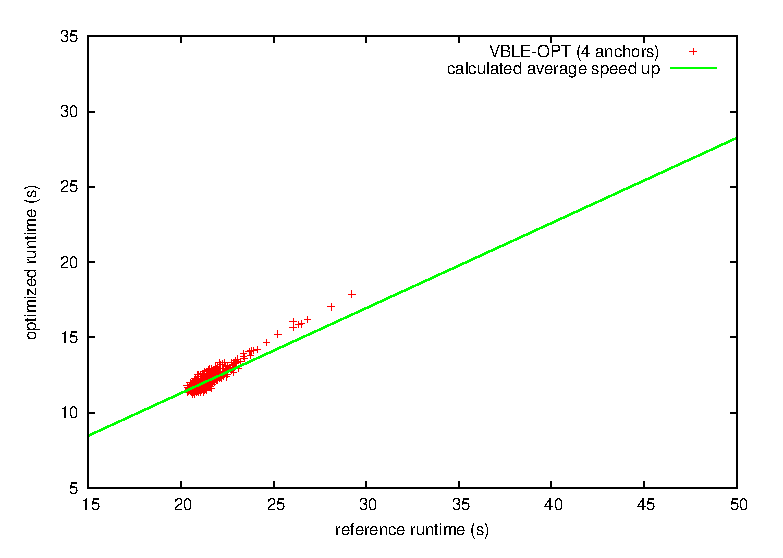
\includegraphics[width=0.75\linewidth]{img/scatter_vble4.eps}
\label{fig:scattervble4}
}
\end{center}
\caption{Benchmark results of VBLE-OPT}
\label{fig:vblescatterplots}
\end{figure}

With regards to Adapted Multilateration, although the speed-up variance is lower than in the case of Geo3, the data has only a weak empiric correlation\footnote{For an introduction to the sample correlation coefficient, see, for example,~\cite[p. 33ff]{ross2004statistics}.} of 0.172, i.e., long reference runtimes did not necessarily result in longer optimized runtimes, and vice versa. This may result from the \emph{first intersection} step occasionally needing more iterations to find circle intersections for all vector elements, in which case the benefits of the vectorization are reduced by the increased processing time spent at the vector comparisons and blending instructions Yet in other runs, the vectorization has larger impacts and runs that were previously slow turned out to have considerable shorter runtimes in the optimized implementation. The scatterplot displayed in Figure~\ref{fig:scatteraml} shows that the speed-up is quite often lower than average (i.e., above the green line), yet there seems to exist no connection between the speed-ups and the original runtimes.

As a concluding remark, I would like to point out that the runtimes of VBLE-OPT using 3 anchors differed measurably from the runtimes of benchmarks using 4 or 5 anchor (or more). Theoretically, the performance of VBLE-OPT should be almost constant with respect to the number of anchors, as the number of cells in the grid is independent of the anchor position and there are no early-out conditionals and the like. Still, when the algorithm was parametrized with 3 anchors, the runtimes varied a lot, yet only towards above the overall average (see Figure~\ref{fig:vblescatterplots}). These slower runs also showed a slightly worse speed-up factor, which resulted in a larger speed-up variance, as depicted in the box-and-whiskers diagram. The reason for these varying runtimes is still unclear to me and could be investigated in future research.
